\chapter{Router con QoS - WRR[1,6]}
\label{chap:conqoswrr16}
\renewcommand{\theenumi}{\alph{enumi}}

\tcolorbox[colback=yellow!20, colframe=yellow!50!black, title=Nota]
En este capítulo, aunque la proporción ya no es la misma como en el caso del WRR[1,1], algunos 
cálculos, como la tasa de entrada en cada cola, es equivalente para ambas, por los que nos 
referimos a una única cola genérica 'Afx', que representa ambas colas de tráfico UDP.
\endtcolorbox

\section{Longitud de cola del router}

\subsection{Mientras dura la transmisión del flujo VoIP}
\begin{enumerate}
    \item Tasa de salida (en pkt/s y b/s) de cada cola AF1x y AF2x:
    \[
        \begin{aligned}
            R_{\text{OutUDP}}[b/s] &= R_{\text{Out}} - R_{\text{OutVoIP}} = 128~\text{kb/s} \cdot 1000~\text{b/kb} - 50~\text{pkt/s} \cdot 199~\text{B/pkt} \cdot 8~\text{b/B} \\
                              &= 48400~\text{b/s} \\
            R_{\text{OutUDP}}[pkt/s] &= 48400~\text{b/s} \cdot \frac{1~\text{B}}{8~\text{b}} \cdot \frac{1~\text{pkt}}{1000~\text{B}} = 6,05~\text{pkt/s} \\ \\
            R_{\text{OutAf1}}[b/s] &= p_{\text{Af1}} \cdot R_{\text{OutUDP}} = \frac{1}{7} \cdot 48400~\text{b/s} = 6914~\text{b/s} \\
            R_{\text{OutAf1}}[pkt/s] &= p_{\text{Af1}} \cdot R_{\text{OutUDP}} = \frac{1}{7} \cdot 6,05~\text{pkt/s} = 0,864~\text{pkt/s} \\ \\
            R_{\text{OutAf2}}[b/s] &= p_{\text{Af2}} \cdot R_{\text{OutUDP}} = \frac{6}{7} \cdot 48400~\text{b/s} = 41486~\text{b/s} \\
            R_{\text{OutAf2}}[pkt/s] &= p_{\text{Af2}} \cdot R_{\text{OutUDP}} = \frac{6}{7} \cdot 6,05~\text{pkt/s} = 5,186~\text{pkt/s} \\
        \end{aligned}
    \]
    En este caso, a diferencia del capítulo anterior (WRR[1,1]), al tener pesos distintos para cada cola,
    la tasa de salida de la cola es mucho mayor en Afx2 que en Afx1.
    \item Paquetes por segundo descartados a la entrada de cada cola:
    \[
        \begin{aligned}
            R_{\text{InAfX}} &= \frac{1~\text{pkt}}{0,08~\text{s}} = 12,5~\text{pkt/s} \\ \\
            Pkt_{\text{DescAf1}} &= R_{\text{InAf1}} - R_{\text{OutAf1}} = 12,5~\text{pkt/s} - 0,864~\text{pkt/s} = 11,636~\text{pkt/s} \\
            Pkt_{\text{DescAf2}} &= R_{\text{InAf2}} - R_{\text{OutAf2}} = 12,5~\text{pkt/s} - 5,186~\text{pkt/s} = 7,314~\text{pkt/s} \\
        \end{aligned}
    \]
    \item Tiempo de llenado de las colas AF1x y AF2x:
    \[
        \begin{aligned}
            t_{\text{FillAf1}} &= \frac{L}{R_{\text{InAf1}} - R_{\text{OutAf1}}} = \frac{100~\text{pkt}}{12,5~\text{pkt/s} - 0,864~\text{pkt/s}} = 8,594~\text{s} \\
            t_{\text{FillAf2}} &= \frac{L}{R_{\text{InAf2}} - R_{\text{OutAf2}}} = \frac{100~\text{pkt}}{12,5~\text{pkt/s} - 5,186~\text{pkt/s}} = 13,672~\text{s} \\
        \end{aligned}
    \]
    Como se observa en la figura \ref{fig:wrr16_tam}, el tiempo de llenado paras las colas UDP es muy 
    bajo, coincidiendo con lo calculado en este apartado.
\end{enumerate}
\begin{figure}[!ht]
    \centering
    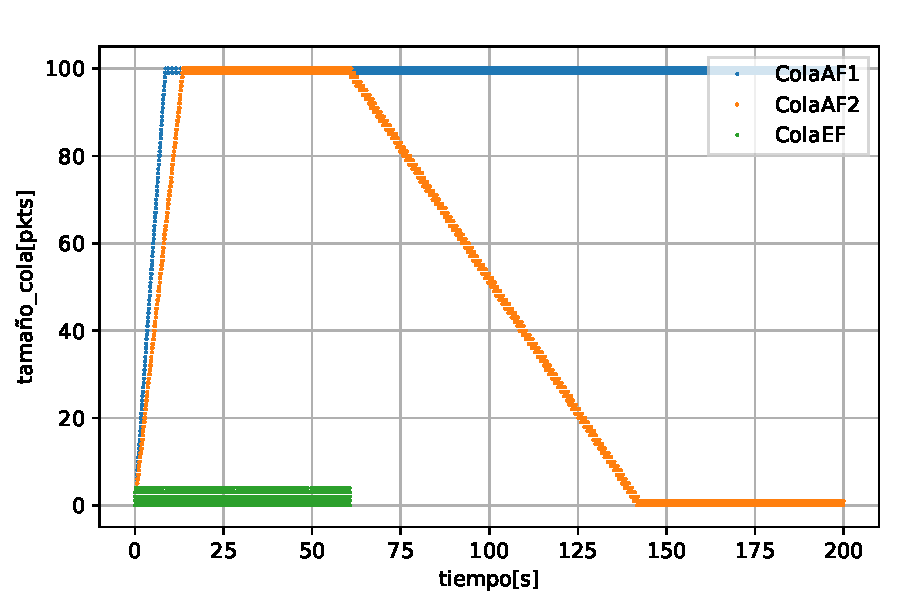
\includegraphics{graficas/WRR/tamao_cola_wrr.pdf}
    \caption{Tamaño de la cola en router con WRR[1,6]}
    \label{fig:wrr16_tam}
\end{figure}

\vspace{0,3cm}

\subsection{Para el caso en el que ya solo se están transmitiendo los dos flujos UDP, calcula la tasa de entrada [pkt/s] y
tasa de salida [pkt/s].}
\[
    \begin{aligned}
        R_{\text{InAfX}} &= \frac{1~\text{pkt}}{0,08~\text{s}} = 12,5~\text{pkt/s} \\ \\
        R_{\text{OutUDP}}[pkt/s] &= 128~\text{kb/s} \cdot 1000~\text{b/kb} \cdot \frac{1~\text{B}}{8~\text{b}} \cdot \frac{1~\text{pkt}}{1000~\text{B}} = 16~\text{pkt/s} \\ \\
        R_{\text{OutAf1}}[pkt/s] &= p_{\text{Af1}} \cdot R_{\text{OutUDP}} = \frac{1}{7} \cdot 16~\text{pkt/s} = 2,286~\text{pkt/s} \\
        R_{\text{OutAf2}}[pkt/s] &= p_{\text{Af2}} \cdot R_{\text{OutUDP}} = \frac{6}{7} \cdot 16~\text{pkt/s} = 13,714~\text{pkt/s} \\
    \end{aligned}
\]
Es interesante fijarse que, para este contexto, al tener un peso de 6, la cola Afx2 se comienza a vaciar 
cuando cesa el flujo VoIP como puede verse con lo que se acaba de calcular (La tasa de salida de Afx2 es mayor 
que la tasa de entrada en la misma). También se refleja en la figura \ref{fig:wrr16_tam}.

\vspace{1cm}

\section{Tiempo en cola del router}
\subsection{Mientras dura la transmisión del flujo VoIP, calcula analíticamente el tiempo en cola de un paquete cuando
la cola AF2x está llena.}
\[
    \begin{aligned}
        t_{\text{qAf2}} &= \frac{L}{R_{\text{OutAf2}}} = \frac{100~\text{pkt}}{5,186~\text{pkt/s}}= 19,283~\text{s} \\
    \end{aligned}
\]
Para comprobar este resultado podemos acudir a la figura \ref{fig:wrr16_time} para ver como el tiempo 
en cola de los paquetes de Afx2 efectivamente se estanca justo antes de los 20s.

\vspace{0,3cm}

\subsection{¿En qué instante entró en la cola AF1x el paquete que salió en t = 60s? ¿Estaba la cola AF1x llena cuando
entró?}
Para realizar este ejercicio nos ayudaremos de la gráfica correspondiente, ya que no es posible 
realizarlo analíticamente, al menos con los conocimientos que tenemos actualmente. Observando 
la figura \ref{fig:wrr16_time} desde Omnet, podemos ver que el paquete saliente de la cola Af1x en el segundo 60, lleva 
en cola un tiempo aproximado de 55,1s.
\[
    \begin{aligned}
        t_{\text{in}} &= t_{\text{out}} - t_{\text{qAf1}} = 60~\text{s} - 55,1~\text{s}= 4,9~\text{s} \\
    \end{aligned}
\]
Por tanto, el momento en el que entró, fue el segundo 4,9. Si nos fijamos en la figura \ref{fig:wrr16_tam}, la cola aún no estaba llena.

\vspace{0,3cm}

\subsection{¿En qué instante salió el primer paquete que se encontró la cola AF1x llena?}
Aunque podría haber forma de obtener un resultado aproximado calculándolo analíticamente, la forma
que se usará para resolver este ejercicio es, igual que en el anterior, la comparación con las gráficas en Omnet.
Primero, acudiremos a la figura \ref{fig:wrr16_tam}. En ella, vemos que el primer paquete que encontró la cola llena
lo hizo en el instante t=8,6s. 
A continuación, debemos buscar el punto en la cola Afx1 de la figura \ref{fig:wrr16_time} en el que,
si  restamos la componente X a la Y, resulte 8,6. Este punto coincidiría con el instante t=84s, momento
en el que salió el primer paquete que encontró la cola llena.

\begin{figure}[!ht]
    \centering
    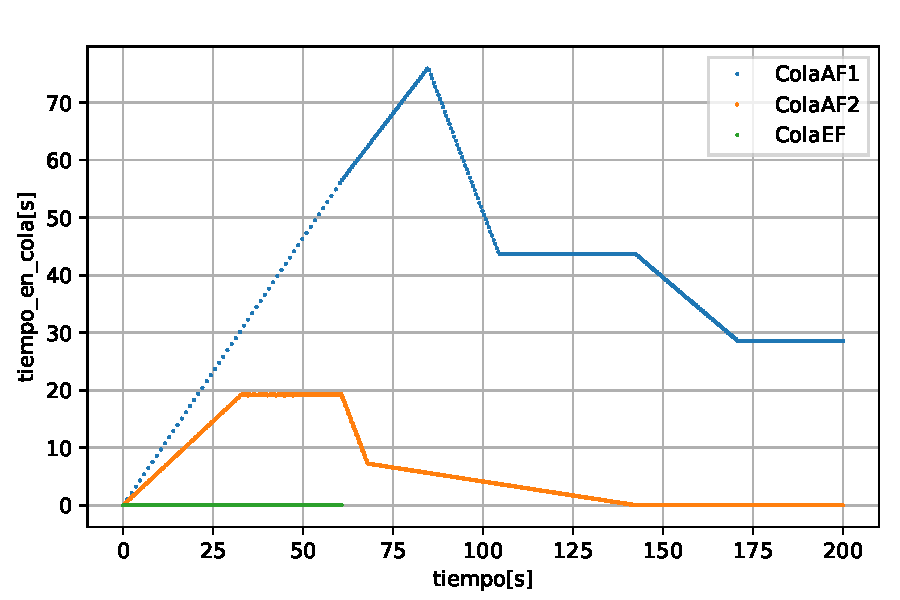
\includegraphics{graficas/WRR/tiempo_en_cola_wrr.pdf}
    \caption{Tiempo en cola de paquetes en router con WRR[1,6]}
    \label{fig:wrr16_time}
\end{figure}

